\subsection{Classification trees}

The following section has the purpose to use tree-based classification methods to find a model which will predict if an NBA's rookie career will be longer than five years.

We started to analyze the data through classification trees using the \textit{gini} minimization function. The result is a complex tree which is difficult to read.

To understand whether it was better to use a simpler tree or not, we performed cross-validation using different levels of tree size and evaluated the impact on the test error.

\Fig~\ref{fig:tree_cv_plot} shows the trends of the deviance and the penalization factor \textit{k} for different values of tree size as determined by cross-validation. In \Fig~\ref{fig:tree_prune_comparison} are shown the obtained trees with different sizes.

\begin{figure}[h]
	\centering
	\begin{subfigure}{.6\textwidth}
		\centering
		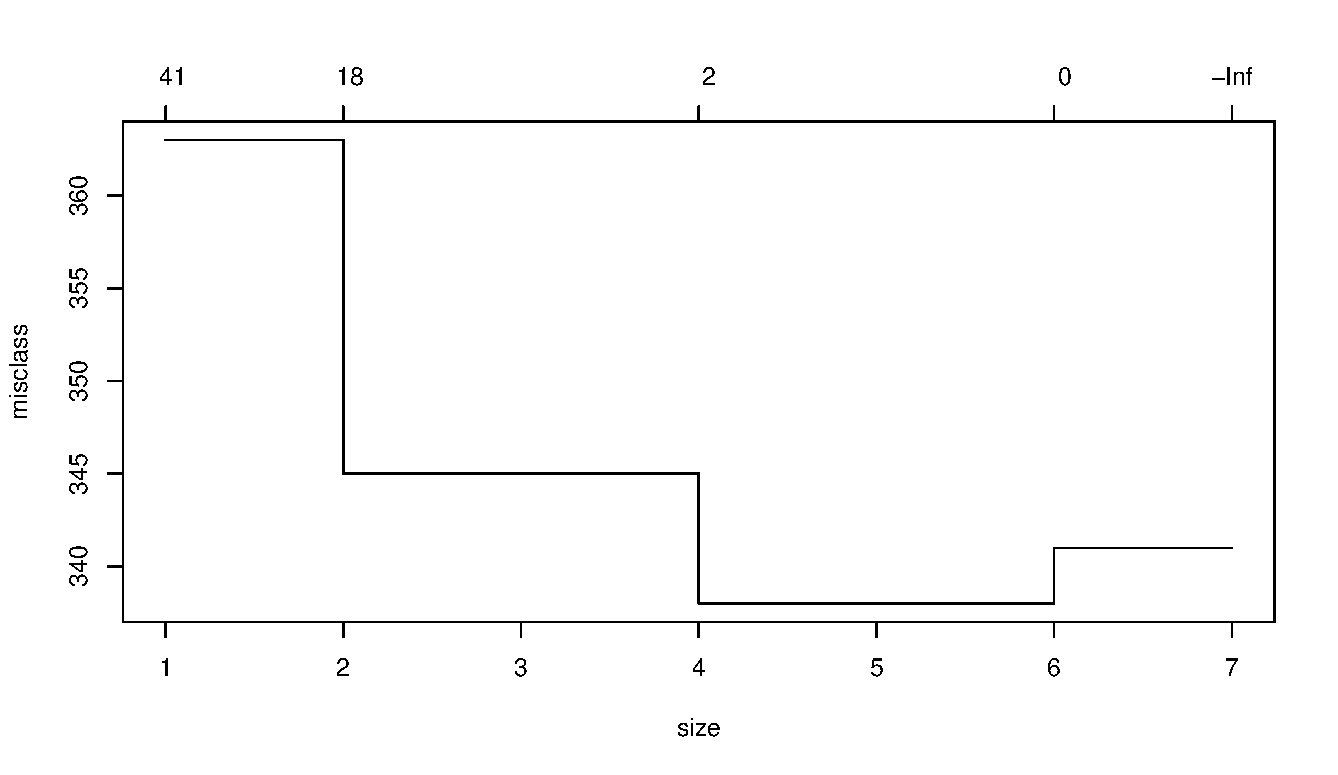
\includegraphics[width=0.5\linewidth]{ImageFiles/Classification/Trees/tree_cv_plot}
		\caption{Size (bottom), deviance (left), k (top).}
		\label{fig:tree_cv_plot}
	\end{subfigure}%
	\begin{subfigure}{.6\textwidth}
		\centering
		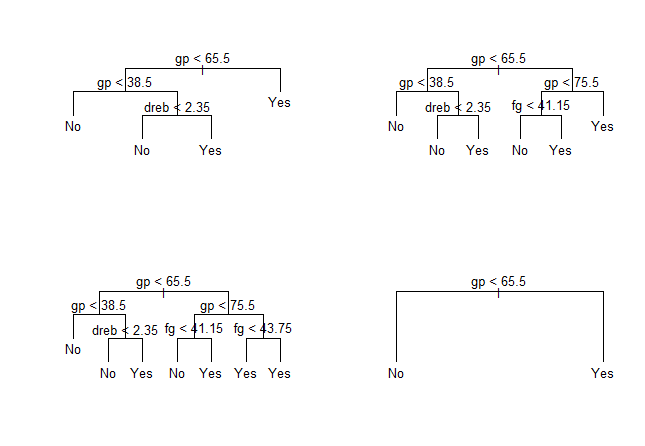
\includegraphics[width=0.5\linewidth]{ImageFiles/Classification/Trees/tree_prune_comparison}
		\caption{Different size trees.}
		\label{fig:tree_prune_comparison}
	\end{subfigure}
	\caption{Obtained trees with various sizes.}
	\label{fig:treeSize}
\end{figure}

After the evaluation of the misclassification error rate on both train and test dataset, we concluded that the best model is the one with $size = 4$.

However, all the trees do the first split on the variable \textit{GP}, suggesting that it is the most important variable.
